\section{基准参数完整扫描与归一化极限}
\label{sec:sup:baseline-scan}
\subsection{代表性控制结果}
本节采用 $N=763,S_0=762,I_0=1,\beta=0.155,\gamma=\delta_q=0.3504\ \mathrm d^{-1},q_0=0.01526$，其余初始仓室为零。常规接触率 $c_0$ 与阈值比例按表\ref{tab:sup:baseline}及各图改变。结果由正文第\ref{sec:s1}节的仅隔离控制解析表达及数值求积得到；$q_{\max}$ 为启动时的隔离比例，$J$ 与总累计新增感染的统计范围沿用本文件开头的约定。
\begin{table}[htbp]
\centering\small
\setlength{\tabcolsep}{3.5pt}
\renewcommand{\arraystretch}{1.25}
\begin{threeparttable}
\caption{基准参数下代表性控制结果}
\label{tab:sup:baseline}
\begin{tabular*}{\linewidth}{@{\extracolsep{\fill}}lS[table-format=2.4]S[table-format=3.4]S[table-format=3.4]S[table-format=1.4]S[table-format=2.4]S[table-format=3.4]@{}}
\toprule
参数取值 & {$t_1$（d）} & {$\Delta t$（d）} & {$t_{\rm end}$（d）} & {$q_{\max}$} & {$J$（d）} & {\shortstack{总累计新增感染\\（人）}}\\
\midrule
\multicolumn{7}{@{}l}{固定 $\eta/N=5\%$，改变 $c_0$}\\
\addlinespace[2pt]
$c_0\approx3.3470$ & 29.9176 & 2.0432 & 71.4690 & 0.0783 & 0.0053 & 382.5525\\
$c_0=4$ & 15.3697 & 6.8658 & 58.7277 & 0.3413 & 0.4374 & 360.7318\\
$c_0=5$ & 9.3039 & 7.5778 & 49.9657 & 0.4946 & 1.0561 & 342.5629\\
$c_0=8$ & 4.3073 & 6.6308 & 38.0095 & 0.6936 & 2.0006 & 303.5829\\
$c_0=10$ & 3.1754 & 5.9026 & 33.7732 & 0.7565 & 2.2236 & 285.7244\\
$c_0=12$ & 2.5150 & 5.3007 & 30.7687 & 0.7978 & 2.3110 & 271.9295\\
\addlinespace[5pt]
\multicolumn{7}{@{}l}{固定 $c_0=10$，改变 $\eta/N$}\\
\addlinespace[2pt]
$\eta/N=0.2\%$ & 0.3602 & 152.0574 & 180.5821 & 0.7734 & 60.8005 & 173.0314\\
$\eta/N=0.6\%$ & 1.3001 & 50.5672 & 86.5579 & 0.7721 & 20.1265 & 195.3349\\
$\eta/N=1\%$ & 1.7406 & 30.2685 & 64.9343 & 0.7708 & 11.9912 & 208.9166\\
$\eta/N=2\%$ & 2.3459 & 15.0431 & 46.8029 & 0.7674 & 5.8888 & 233.7810\\
\bottomrule
\end{tabular*}
\begin{tablenotes}[flushleft]\footnotesize
\item 注：表中列出仅隔离控制的结果；首行 $c_0=c_{0,\min}+0.02$，近似数不作重新求解的输入。第一组阈值为 $5\%$；正文多阈值曲线另取 $0.2\%,0.6\%,1\%,2\%$。
\end{tablenotes}
\end{threeparttable}
\end{table}
\subsection{归一化低阈值极限}
若固定 $i_0>0$，允许的阈值为 $\theta>i_0$，不能直接在这一固定初值问题中令 $\theta\to0$。沿同时满足 $i_0\to0$、$\theta\to0$、$0<i_0<\theta$ 的序列，且 $s_0$ 趋于某个大于 $s_c$ 的固定值时，有 $s^*\to s_0$，从而
\begin{equation}
\Delta t\sim\frac1{c_0\theta}\ln\frac{s_0-\bar s}{s_c-\bar s},\qquad
J\sim\frac2{c_0\theta}\int_{s_c}^{s_0}\frac{(1-s_c/s)^2}{s-\bar s}\,ds.
\label{eq:small-threshold}
\end{equation}
两者均按 $1/\theta$ 的量级发散。相反，在固定 $i_0>0$ 时令 $\theta\downarrow i_0$，控制时长趋于有限值
\[
\frac1{c_0i_0}\ln\frac{s_0-\bar s}{s_c-\bar s}.
\]
因此，基于时长或成本反函数定义的阈值边界应限定在相应值域内；不能将联合小初值极限用于固定正初值的反函数结论。


% ===== 04_numerical_illustrations =====
\subsection{参数敏感性的数值图示}
参数取值见各图图注。图\ref{fig:baseline:q-joint}给出不同 $c_0$ 与 $\eta$ 下的隔离比例轨迹。图\ref{fig:scenario1_heatmaps_c0_eta}则展示相关指标在同一参数平面内的变化；触发边界下方无需加强隔离。代表数值见正文第\ref{sec:numerics}节及补充表\ref*{tab:sup:baseline}。

\begin{figure}[htbp]
\centering
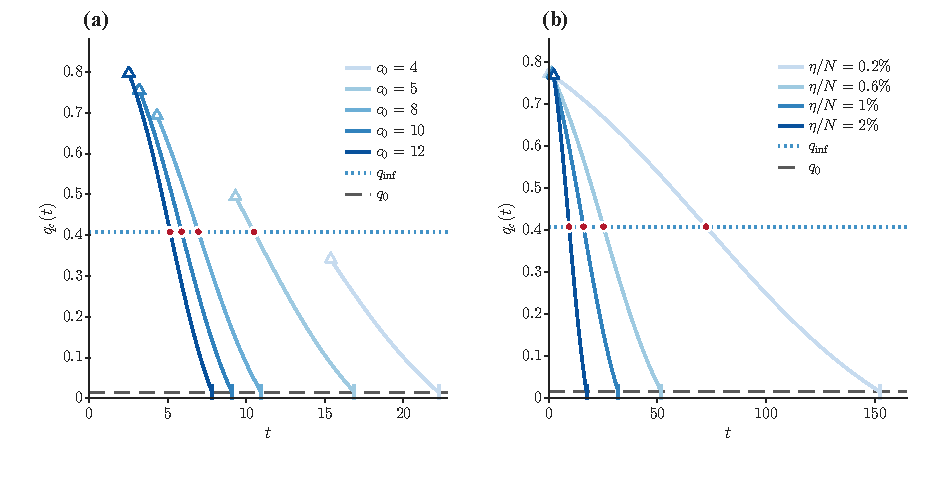
\includegraphics[width=\textwidth]{figures/layout_v5/baseline_q_joint.pdf}
\caption{不同常规接触率和感染阈值下的隔离比例轨迹。固定 $N=763,S_0=762,I_0=1,\beta=0.155,\gamma=0.3504\ \mathrm d^{-1},q_0=0.01526$。(a) 固定 $\eta/N=5\%$，$c_0=4,5,8,10,12$；(b) 固定 $c_0=10$，$\eta/N=0.2\%,0.6\%,1\%,2\%$。三角形、短竖线分别表示 $t_1,t_2$，红点为内部拐点。水平虚线为 $q_0$，点线为 $\qinf$。$c_0=4$ 时不存在内部拐点。横轴 $t$ 的单位为天。}
\label{fig:baseline:q-joint}
\end{figure}

\begin{figure}[htbp]
\centering
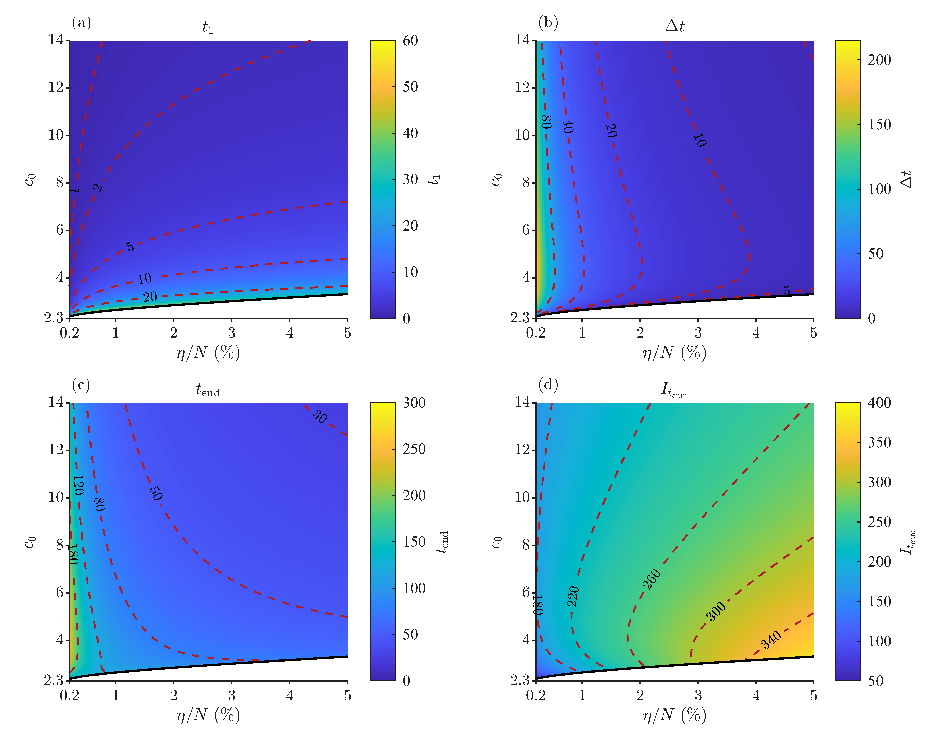
\includegraphics[width=0.8\textwidth]{figures/scenario1_heatmaps_c0_eta.pdf}
\caption{$(\eta/N,c_0)$ 平面上的启动时间、控制时长、清零时间和累计新增感染。固定 $N=763,S_0=762,I_0=1,\beta=0.155,\gamma=0.3504\ \mathrm d^{-1},q_0=0.01526$。实线为触发边界 $c_{0,\min}(\eta)$，白色区域无需加强隔离，虚线为各指标的等值线。}
\label{fig:scenario1_heatmaps_c0_eta}
\end{figure}


\FloatBarrier

